%!TEX root = thesis.tex

\chapter{Follow-Up User Study}
\label{chap:follow-up-user-study}

A follow-up user study was conducted to evaluate the set of refined visualisations.

\section{Method}

Two independent audiences ($N=14+11=25$) were recruited
The hypothesis for this study was that visualisations would result in higher understanding at the end of the performance and that enjoyment would remain equally steady throughout both performances.

\section{Participants}

A total of 25








\section{Results}


\subsection{Enjoyment}

\afterpage{
\begin{figure}
  \centering
  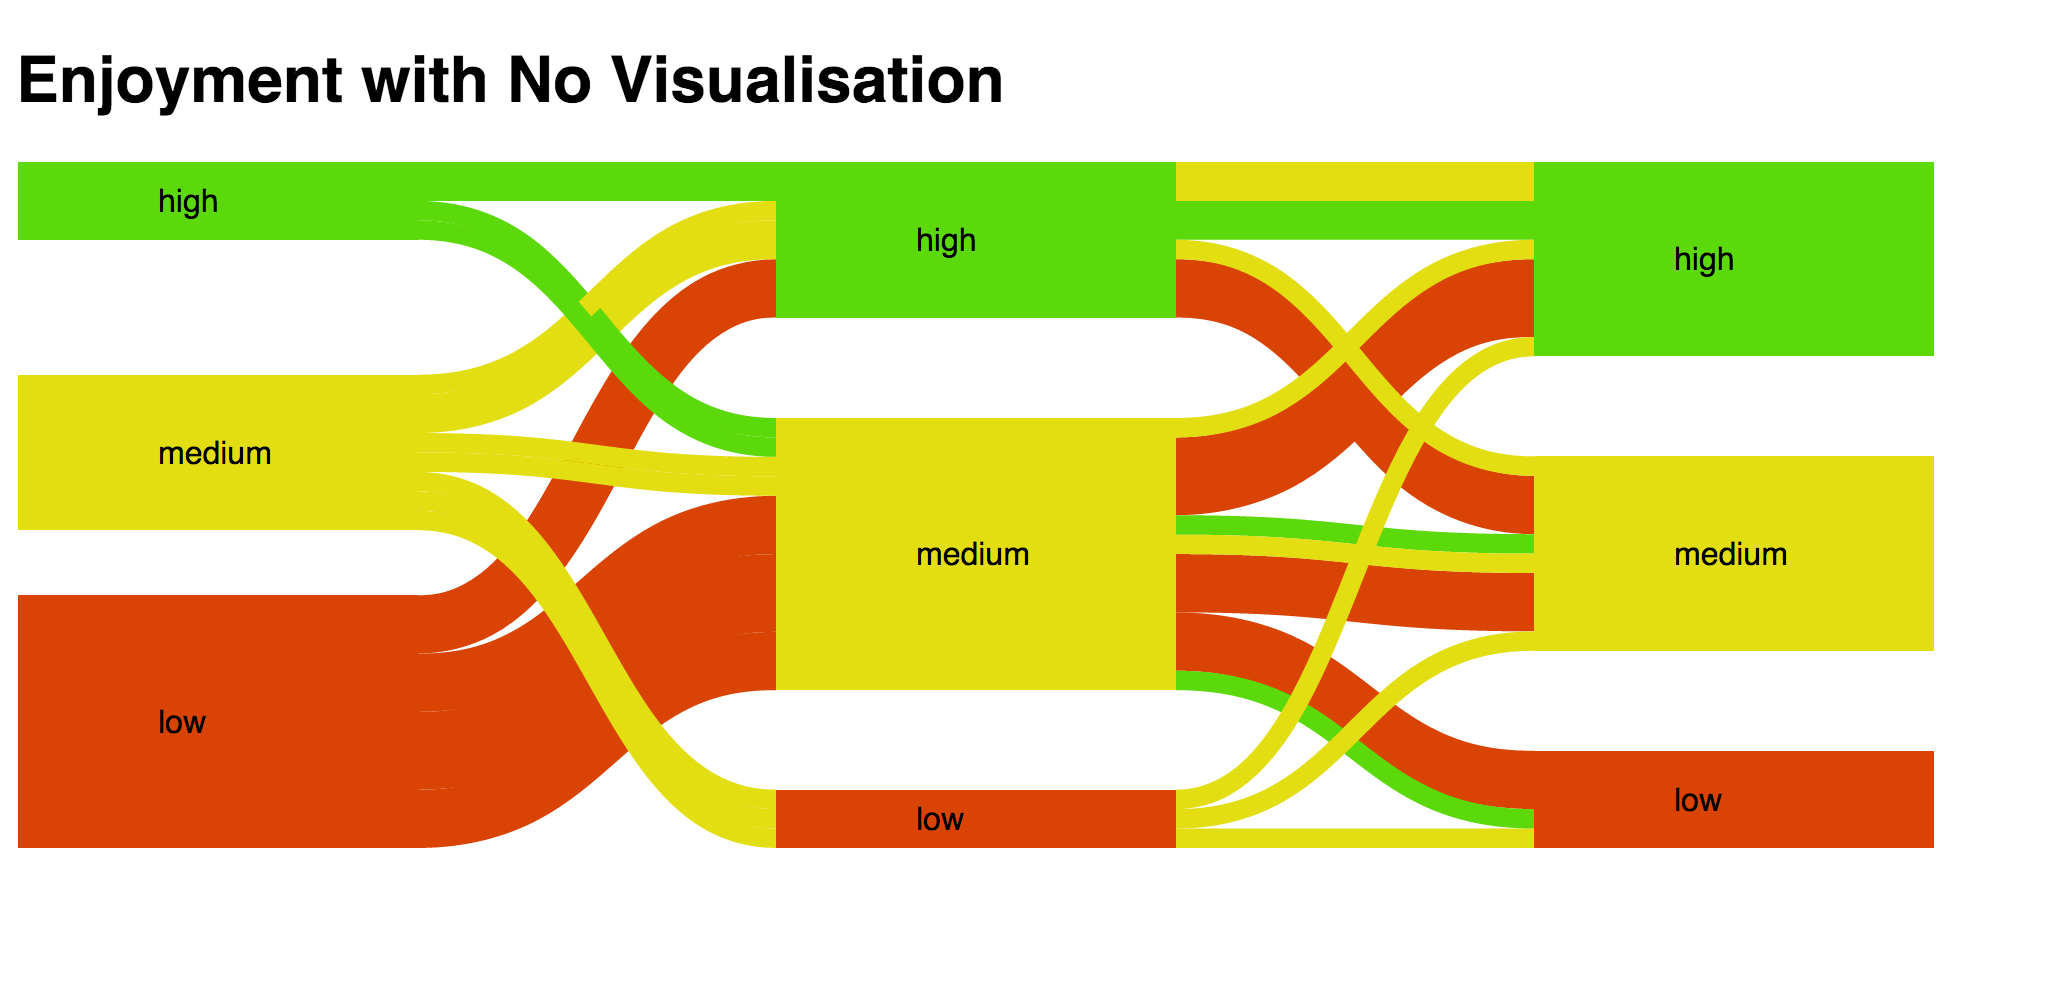
\includegraphics[width=\columnwidth]{../study-3/results/enjoyment-with-no-visualisation-study-3}
  \caption{Audience reported enjoyment during the beginning, middle and end of the performance with \textbf{no} visualisations. Line width at each stage indicates proportion of the audience reporting high, medium or low enjoyment, and line colour is determined by the enjoyment level at the \emph{beginning} of the performance.}
  \label{fig:no-visualisations-enjoyment}
\end{figure}

\begin{figure}
  \centering
  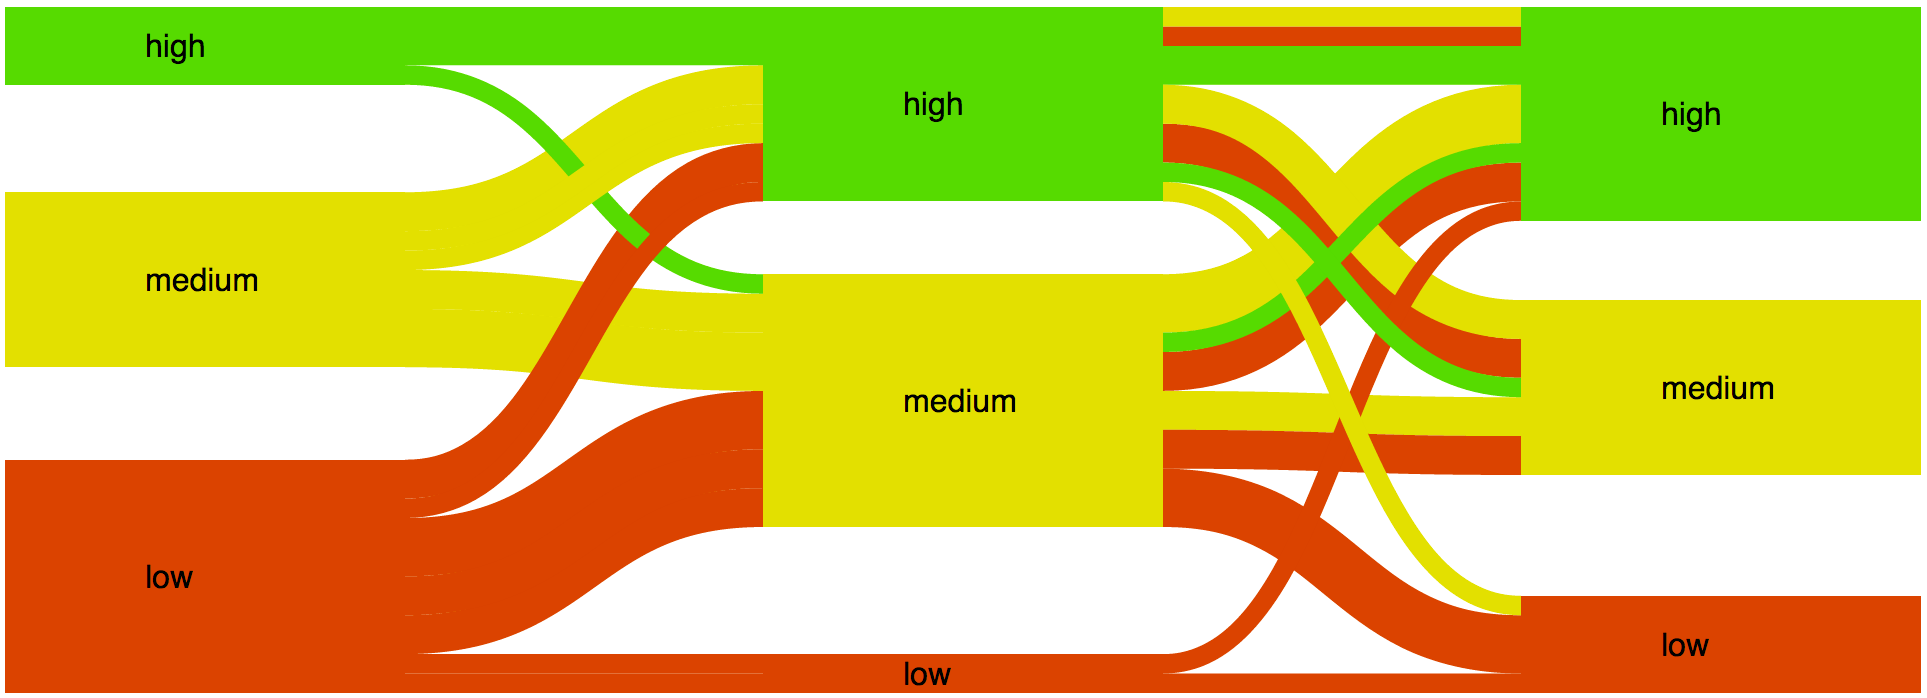
\includegraphics[width=\columnwidth]{../study-3/results/enjoyment-with-visualisation-study-3}
  \caption{Audience-reported enjoyment level during the beginning, middle and end of the performance with visualsations.}
  \label{fig:visualisations-enjoyment}
\end{figure}
\clearpage}

\subsection{Understanding}

\afterpage{
\begin{figure}
  \centering
  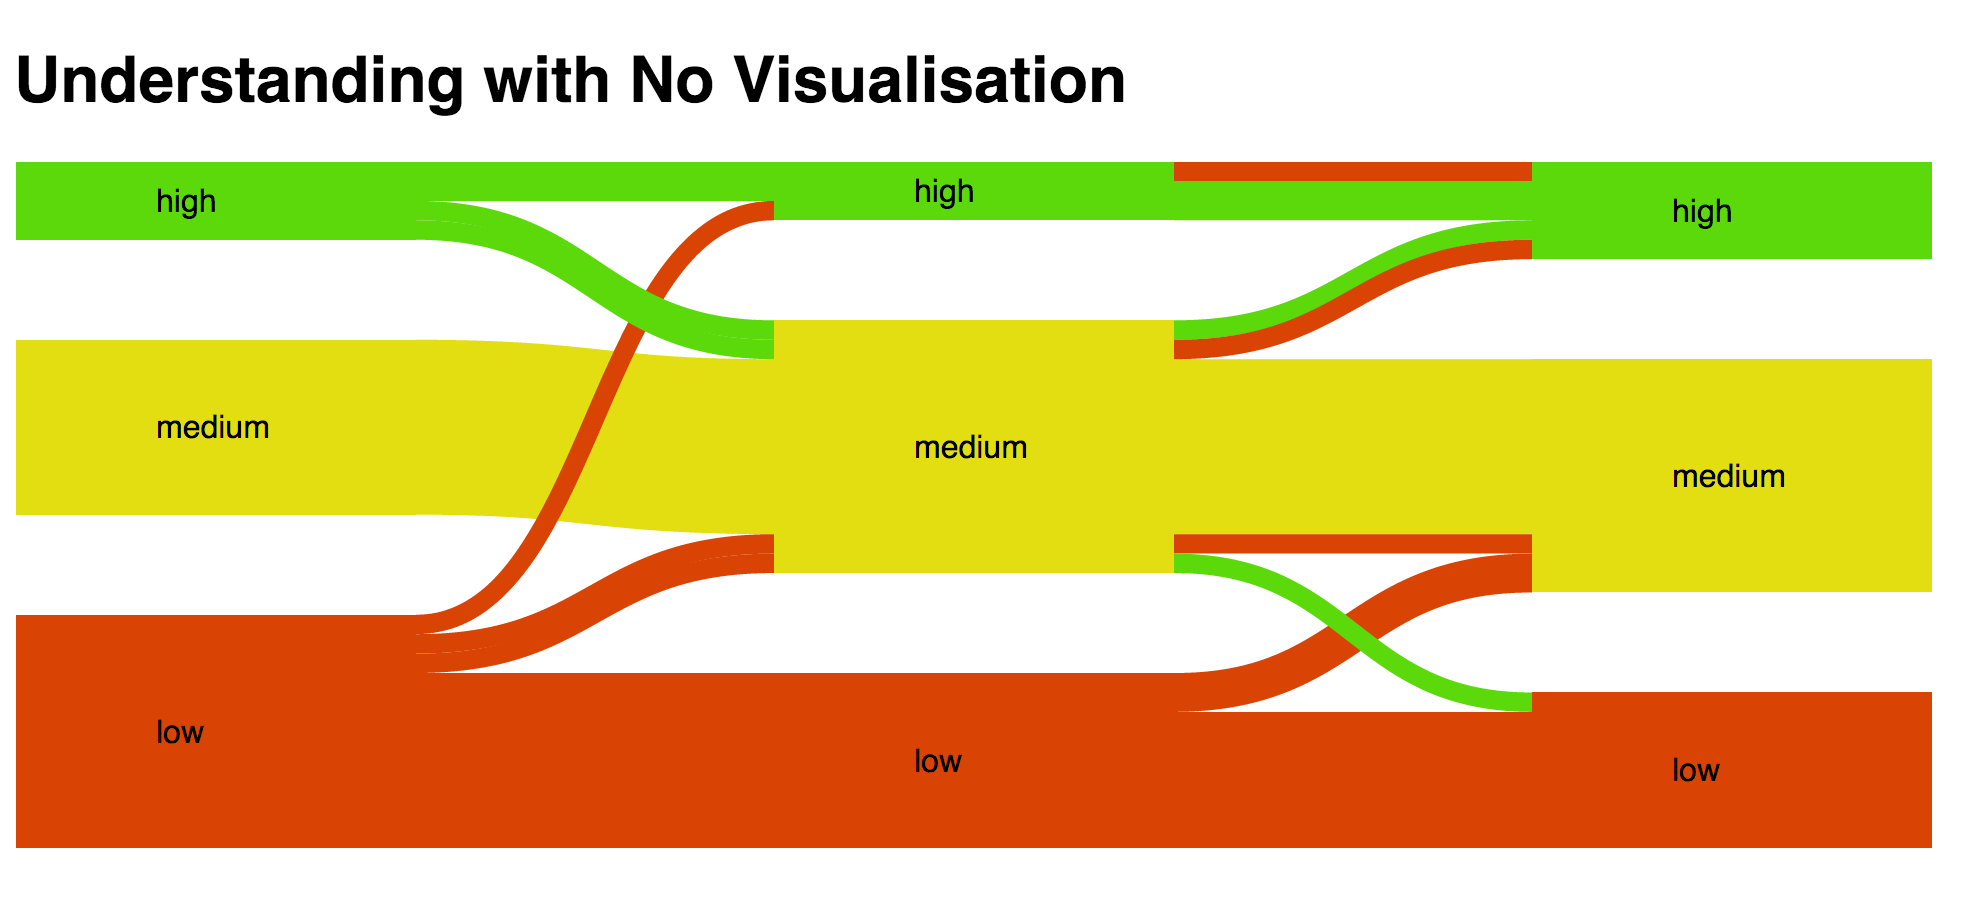
\includegraphics[width=\columnwidth]{../study-3/results/understanding-with-no-visualisation-study-3}
  \caption{Audience reported understanding during the beginning, middle and end of the performance with \textbf{no} visualisations.}
  \label{fig:no-visualisations-understanding}
\end{figure}

\begin{figure}
  \centering
  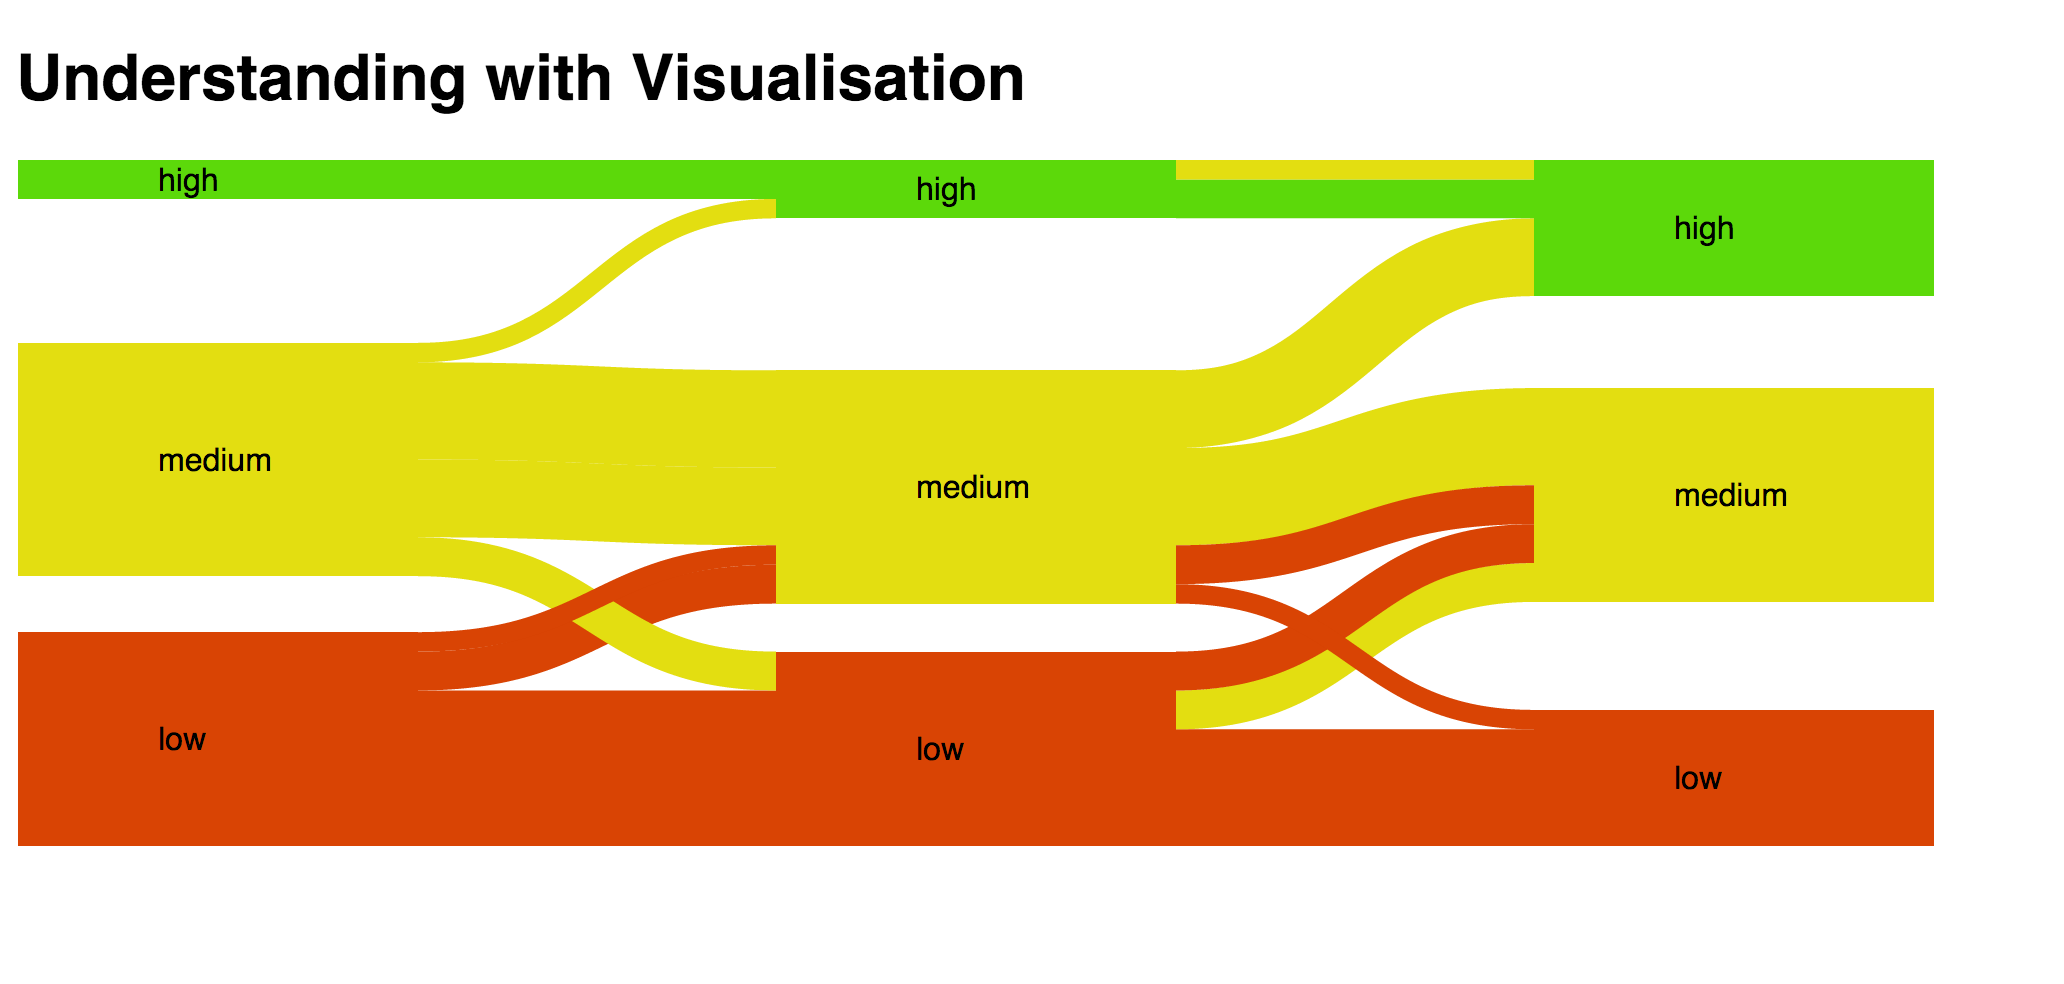
\includegraphics[width=\columnwidth]{../study-3/results/understanding-with-visualisation-study-3}
  \caption{Audience reported understanding during the beginning, middle and end of the performance with visualisations.}
  \label{fig:visualisations-understanding}
\end{figure}

\clearpage}

\section{Discussion}





\subsection{Validity}

\subsection{Limitations}



\section{Summary}










